\documentclass[aps,prl,reprint,superscriptaddress,showpacs,floatfix]{revtex4-2}
\usepackage{graphicx}
\usepackage{amsmath}
\usepackage{amssymb}
\usepackage{xcolor}
\usepackage[colorlinks=true, breaklinks=true, linkcolor=blue, citecolor=blue, urlcolor=blue]{hyperref}

\begin{document}

\title{Intrinsic Information Limit in Nuclear Optical Potential Extraction}

\author{Jin Lei}
\email{jinl@tongji.edu.cn}
\affiliation{School of Physics Science and Engineering, Tongji University, Shanghai 200092, China}
\affiliation{Southern Center for Nuclear-Science Theory (SCNT), Institute of Modern Physics, Chinese Academy of Sciences, Huizhou 516000, Guangdong Province, China}

\date{\today}

\begin{abstract}
How many independent parameter combinations can nucleon-nucleus scattering data actually constrain in the optical model potential? Using the effective dimensionality $D_\mathrm{eff}$ (the participation ratio of Fisher information eigenvalues), I show that, within the Koning-Delaroche (KD02) framework, the continuous ``Igo ambiguity'' reflects a structural information bottleneck rather than insufficient data. Single-energy elastic scattering constrains only $D_\mathrm{eff} \approx 1.7 \pm 0.4$ parameter combinations (averaged over 168 configurations spanning $A = 12$--$208$, $E = 10$--$200$~MeV, and both projectile types). Decomposing how each data class redistributes the Fisher spectrum reveals a clear hierarchy for opening independent parameter directions: systematic multi-energy fitting within the KD02 energy dependence gives the largest increase ($D_\mathrm{eff} \to \sim\!2.3$--$2.5$ in the 13-parameter local space; $D_\mathrm{eff} \approx 2.9$ out of 48 universal KD02 coefficients), the analyzing power $A_y$ gives the next-largest increase for most neutron configurations at representative precision ratios, while $\sigma_R$ alone opens essentially no new direction. This bottleneck is stable across the configurations sampled: uniform error reduction rescales the local Fisher spectrum without changing its anisotropy, whereas qualitatively different measurements can partially broaden it. For downstream reaction calculations, this identifies which optical-potential directions must be pinned or propagated before discrepancies are assigned to reaction or structure physics. In logarithmic KD02 coordinates, the spectrum has the standard local signature of a ``sloppy model,'' and the analysis provides a systematic effective-dimensionality map of the Igo ambiguity.
\end{abstract}

\pacs{24.10.Ht, 25.40.Cm, 02.50.Tt}

\maketitle

%=====================================================
% INTRODUCTION
%=====================================================
\textit{Introduction.}---Direct reactions on weakly bound and rare isotopes infer structure and response information through optical potentials that are not observables themselves. When a transfer, breakup, or charge-exchange calculation disagrees with data, the first diagnostic question is whether the discrepancy originates in the optical interaction, the reaction mechanism, or the structure input. This question reaches back to the inception of the optical model potential (OMP) over seventy years ago~\cite{Feshbach1954,Feshbach1958,Feshbach1962}. Since then, the OMP has become the effective interaction behind much of nuclear reaction theory~\cite{Hodgson1971,Satchler1983,Mahaux1991,Dickhoff2019}, but a basic inverse-problem obstruction persists: the ``inverse problem ill-posedness,'' historically known as the Igo ambiguity~\cite{Igo1958}. Distinct parameter sets, representing different nuclear potentials, can yield indistinguishable scattering cross sections~\cite{Perey1976,Greenlees1968}, creating a continuous degeneracy that an elastic fit alone cannot resolve.

Two types of ambiguity exist~\cite{Satchler1983}: \emph{discrete} ambiguity from different wavefunction node numbers (resolvable by high-energy rainbow scattering), and \emph{continuous} ambiguity where parameters trade off while maintaining the potential near the nuclear surface~\cite{Greenlees1968}. For a Woods-Saxon potential, this surface sensitivity is captured by the volume integral $J_V \propto V r_v^3$~\cite{Satchler1983}. The qualitative origin of this continuous ambiguity is well understood: elastic scattering is primarily sensitive to the potential near the nuclear surface, making it insensitive to the detailed radial shape~\cite{Satchler1983}. However, despite this qualitative understanding, three key questions lack quantitative answers: (1)~\emph{How many} independent parameter combinations can actually be constrained? (2)~Can improved experimental precision eventually resolve the degeneracy? (3)~Is the ambiguity universal across the nuclear chart?

Recent Bayesian uncertainty quantification~\cite{Furnstahl2015,Phillips2021} has documented large parameter uncertainties in nuclear reaction models. The motivation goes beyond attaching error bars to optical-model fits: in transfer, breakup, charge-exchange, and other reactions involving weakly bound or rare isotopes, a disagreement with data cannot be interpreted until the error budget separates optical-potential input from reaction-mechanism approximations, structure overlaps, and missing channels~\cite{King2018,Lovell2021}. This need is explicit in the rare-isotope-beam literature, where quantifying and reducing reaction-model uncertainties, especially those associated with nuclear optical potentials, has been identified as a targeted priority~\cite{Hebborn2023}. King \textit{et al.}~\cite{King2019PRL} showed that Bayesian MCMC posterior distributions for optical potential parameters are strongly non-Gaussian, with only the depth $V$ and radius $r_v$ strongly correlated, whereas the frequentist $\chi^2$ approach produced spurious correlations among many parameter pairs. Subsequent studies confirmed these findings~\cite{King2018,Lovell2021,Catacora2019}, while principal component analysis identified the dominant variance directions~\cite{Catacora2021}. Yet these empirical observations require $\sim$100,000 MCMC samples per system for converged correlation studies and lack a theoretical framework that would answer the questions above.

In this Letter, I address these questions quantitatively using Fisher information geometry~\cite{Fisher1925}, focusing on the continuum regime ($E = 10$--$200$~MeV), above the resonance region where smooth optical potentials such as KD02 are designed to apply. In logarithmic KD02 coordinates and for the stated error models, the eigenvalue spectra have the standard signature of ``sloppy models''~\cite{Waterfall2006PRL,Gutenkunst2007,Machta2013,Transtrum2015,Niksic2016}: only a few ``stiff'' (large eigenvalue) parameter combinations are well constrained, while the remaining directions are ``sloppy'' (data-insensitive). This is a local spectral classification, not a requirement that published best-fit parameters drift by orders of magnitude; physical constraints, shared parameter relations, and global systematics can pin directions that one observable class leaves flat. By systematically scanning 168 configurations across the nuclear chart and progressively adding observables, I establish the stability of this bottleneck and identify which data classes open independent parameter directions beyond elastic scattering.

%=====================================================
% METHOD
%=====================================================
\textit{Method.}---Consider nucleon-nucleus elastic scattering with the Koning-Delaroche (KD02) global optical potential~\cite{Becchetti1969,Varner1991,Koning2003}, which has 9 parameters for the central terms: real volume $(V, r_v, a_v)$, imaginary volume $(W, r_w, a_w)$, and imaginary surface $(W_d, r_d, a_d)$. Including spin-orbit coupling with Thomas form adds 4 parameters $(V_{so}, W_{so}, r_{so}, a_{so})$, yielding a 13-parameter model for spin-1/2 scattering. (Although KD02 constrains $r_w = r_v$ and $a_w = a_v$, I retain them as independent in the Fisher analysis to test whether data could in principle distinguish them; see End Matter.)

The \emph{relative sensitivity} of the differential cross section $\sigma(\theta) \equiv d\sigma/d\Omega(\theta)$ to each parameter $p_i$ is
\begin{equation}
S_i(\theta) = \frac{\partial \log \sigma(\theta)}{\partial \log p_i} = \frac{p_i}{\sigma} \frac{\partial \sigma}{\partial p_i}.
\end{equation}
Using logarithmic derivatives makes parameters with different physical units directly comparable. Working in logarithmic parameter space throughout, the Fisher information matrix~\cite{Fisher1925} (FIM) for a data vector $\{y_k\}$ with uncertainties $\{\delta_k\}$ is
\begin{equation}
F_{ij} = \sum_k \delta_k^{-2}\,\frac{\partial y_k}{\partial \log p_i}\frac{\partial y_k}{\partial \log p_j},
\end{equation}
where $\partial y_k / \partial \log p_i = p_i\,\partial y_k / \partial p_i$. For elastic cross sections with uniform relative uncertainties $\delta_k = \epsilon\,\sigma(\theta_k)$, this reduces to $F_{ij} = \epsilon^{-2} \sum_\theta S_i(\theta)\, S_j(\theta)$. The overall factor $\epsilon^{-2}$ cancels in $D_\mathrm{eff}$ (see below), so the information structure depends only on the sensitivity matrix $S_i(\theta)$, evaluated at the KD02 reference parameter values for each $(A, Z, E)$ configuration, using 35 scattering angles equally spaced from $5^\circ$ to $175^\circ$. For $A_y$, absolute uncertainties are used ($\delta_{A_y} = 0.03$); for $\sigma_R$ and $\sigma_T$, uniform relative uncertainties are assumed ($\sigma_T$ enters for neutron projectiles only, since the Coulomb divergence of $f(0)$ leaves it undefined for protons). Only the \emph{relative weighting} between observable types, set by $\epsilon / \delta_{A_y}$, therefore affects the result: the combined-observable results below use $\epsilon = 1$ and $\delta_{A_y} = 0.03$, and the quantitative $A_y$ gain depends on this ratio (see End Matter), while the qualitative hierarchy is robust. $D_\mathrm{eff}$ thus responds to the \emph{structure} of the error model (relative vs.\ absolute, angular coverage), not to its overall magnitude. Each observable type enters additively ($F = F_\mathrm{elastic} + F_{A_y} + \cdots$), enabling the step-by-step decomposition below.

Diagonalizing the FIM yields eigenvalues $\lambda_1 \geq \lambda_2 \geq \cdots \geq \lambda_{N_p}$ and corresponding unit eigenvectors $\mathbf{e}_i$ in the $N_p$-dimensional space of (log-)parameters, where $N_p$ is the number of parameters: $\lambda_i$ quantifies how much information the data carry along $\mathbf{e}_i$, and the squared component $e_{i,k}^2$ gives the fractional contribution of parameter $p_k$ to that mode. The effective dimensionality, defined as the participation ratio~\cite{Bell1970,Gutenkunst2007} of the FIM eigenvalues,
\begin{equation}
D_\mathrm{eff} = \frac{(\sum_i \lambda_i)^2}{\sum_i \lambda_i^2},
\end{equation}
ranges from 1 (one direction dominates) to the total number of parameters (all directions equally constrained); $D_\mathrm{eff} \approx 2$ does not mean that only 2 directions carry \emph{any} information, but rather that information is overwhelmingly concentrated in $\sim$$D_\mathrm{eff}$ stiff modes. $D_\mathrm{eff}$ is \emph{scale-invariant}: reducing all experimental errors by the same factor scales every $\lambda_i$ uniformly, leaving $D_\mathrm{eff}$ unchanged. Only qualitatively different measurements (e.g., adding $A_y$ to $d\sigma/d\Omega$) can alter $D_\mathrm{eff}$ by changing the relative eigenvalue spectrum (see End Matter for a concrete illustration). The use of logarithmic derivatives further ensures invariance under parameter rescaling $p_i \to c_i\,p_i$, so that $V$ (in MeV) and $r_v$ (in fm) enter on an equal footing. Numerical details are given in the End Matter.

%=====================================================
% RESULTS
%=====================================================
\textit{Results.}---I systematically analyze 168 configurations: 12 nuclei ($^{12}$C to $^{208}$Pb), 7 energies (10--200~MeV), and both neutron and proton projectiles. Figure~\ref{fig:deff_universal} displays $D_\mathrm{eff}$ as a heatmap across all configurations. The uniformity ($D_\mathrm{eff}$ typically 1--2, with occasional values reaching $\sim$3 for light nuclei at high energy) demonstrates that the information limit is stable across the configurations sampled, with only weak dependence on target mass, beam energy, or projectile type. The statistics yield $D_\mathrm{eff} = 1.59 \pm 0.29$ (neutrons) and $1.73 \pm 0.47$ (protons), with a combined average of $1.7 \pm 0.4$ over all 168 configurations. The physical origin of this stability is that elastic scattering is primarily sensitive to the nuclear surface geometry (the potential radius scale) for every nucleus and beam energy sampled, as confirmed by the eigenvector analysis below.

\begin{figure}[t]
\centering
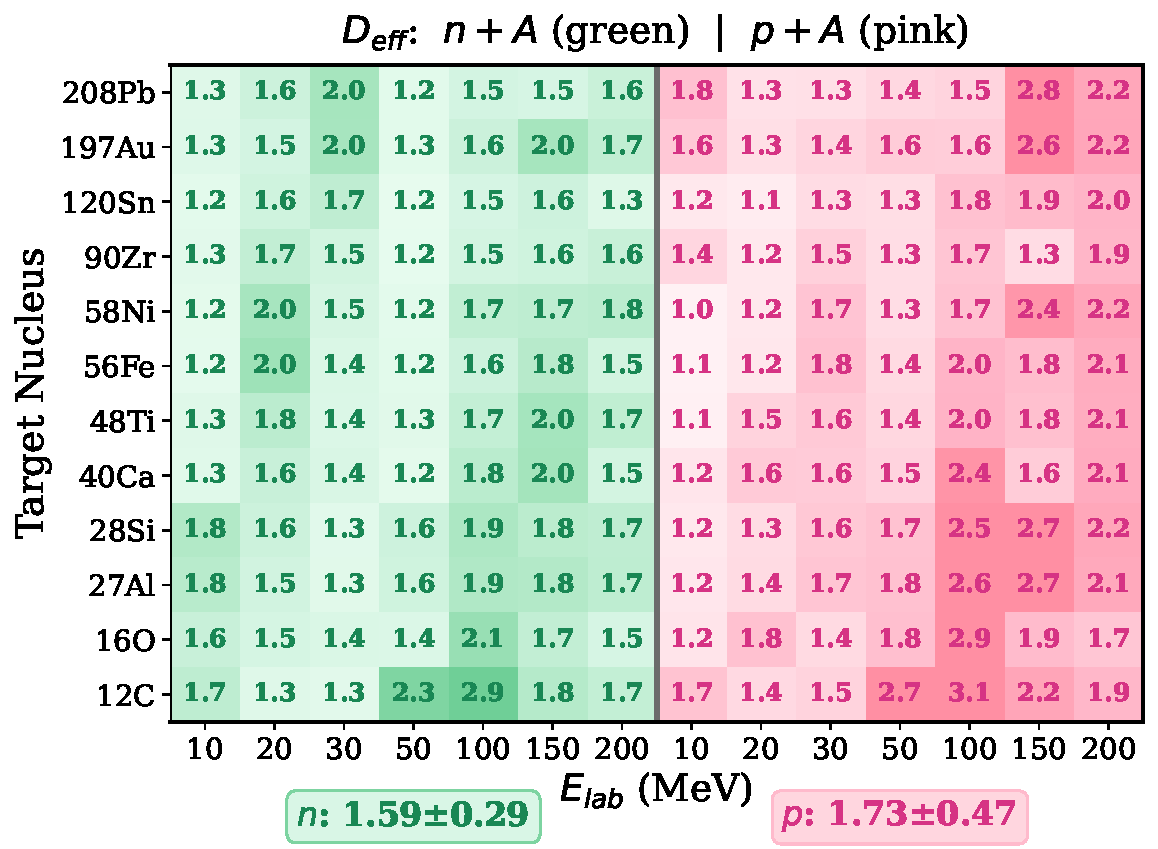
\includegraphics[width=\columnwidth]{fig1_deff_universal.pdf}
\caption{Effective dimensionality $D_\mathrm{eff}$ for single-energy elastic scattering across 12 nuclei and 7 energies for neutron (green) and proton (pink) projectiles. Values typically range from 1 to 2 (occasionally reaching $\sim$3), showing that only $\sim$2 out of 13 KD02 parameter combinations are effectively constrained for every target and beam energy sampled.}
\label{fig:deff_universal}
\end{figure}

Complementary cuts through the same scan (see End Matter, Fig.~\ref{fig:deff_combined}) confirm this stability: $D_\mathrm{eff}$ stays within 1.1--2.4 from $^{12}$C to $^{208}$Pb at 50~MeV, bounded between 1 and 3 across all energies, with condition numbers $\kappa = \lambda_\mathrm{max}/\lambda_\mathrm{min}$ of $10^6$ to above $10^{10}$ rendering the $\sim$11 sloppy dimensions effectively unobservable.

\textit{Anatomy of the information limit.}---Figure~\ref{fig:eigenvectors} shows the eigenvector composition for $n+^{40}$Ca at 50~MeV. The dominant mode $\mathbf{e}_1$ (90\% of information) is driven by $r_v$ (62\%), $r_d$ (14\%), and $V$ (11\%), corresponding to the volume integral $J_V \propto V r_v^3$; the signed eigenvector components show $r_v$ and $V$ entering with the same sign. If the data measured $J_V$ alone, the stiff eigenvector would be the gradient of $\log J_V$, with squared weights of 10\% ($V$) and 90\% ($r_v$); the computed $\mathbf{e}_1$ matches this direction, diluted by the $r_d$ admixture. The radius $r_v$ dominates because $\partial\log J_V/\partial\log r_v = 3$ versus $\partial\log J_V/\partial\log V = 1$. The Igo ambiguity~\cite{Igo1958} corresponds to the perpendicular direction in the $V$-$r_v$ plane: increasing $V$ while decreasing $r_v$ (or vice versa) keeps $J_V$ approximately constant, leaving the cross section nearly unchanged. Along this direction the Fisher information is roughly a factor of 50 smaller than along $\mathbf{e}_1$. The second mode $\mathbf{e}_2$ (7\%) mixes $r_v$ (29\%), $a_v$ (27\%), and $r_d$ (24\%), encoding the radial geometry. Together, these two modes capture 97\% of all information; the remaining 11 directions, including diffuseness, imaginary potential, and spin-orbit, are effectively invisible to elastic angular distributions.

\begin{figure}[t]
\centering
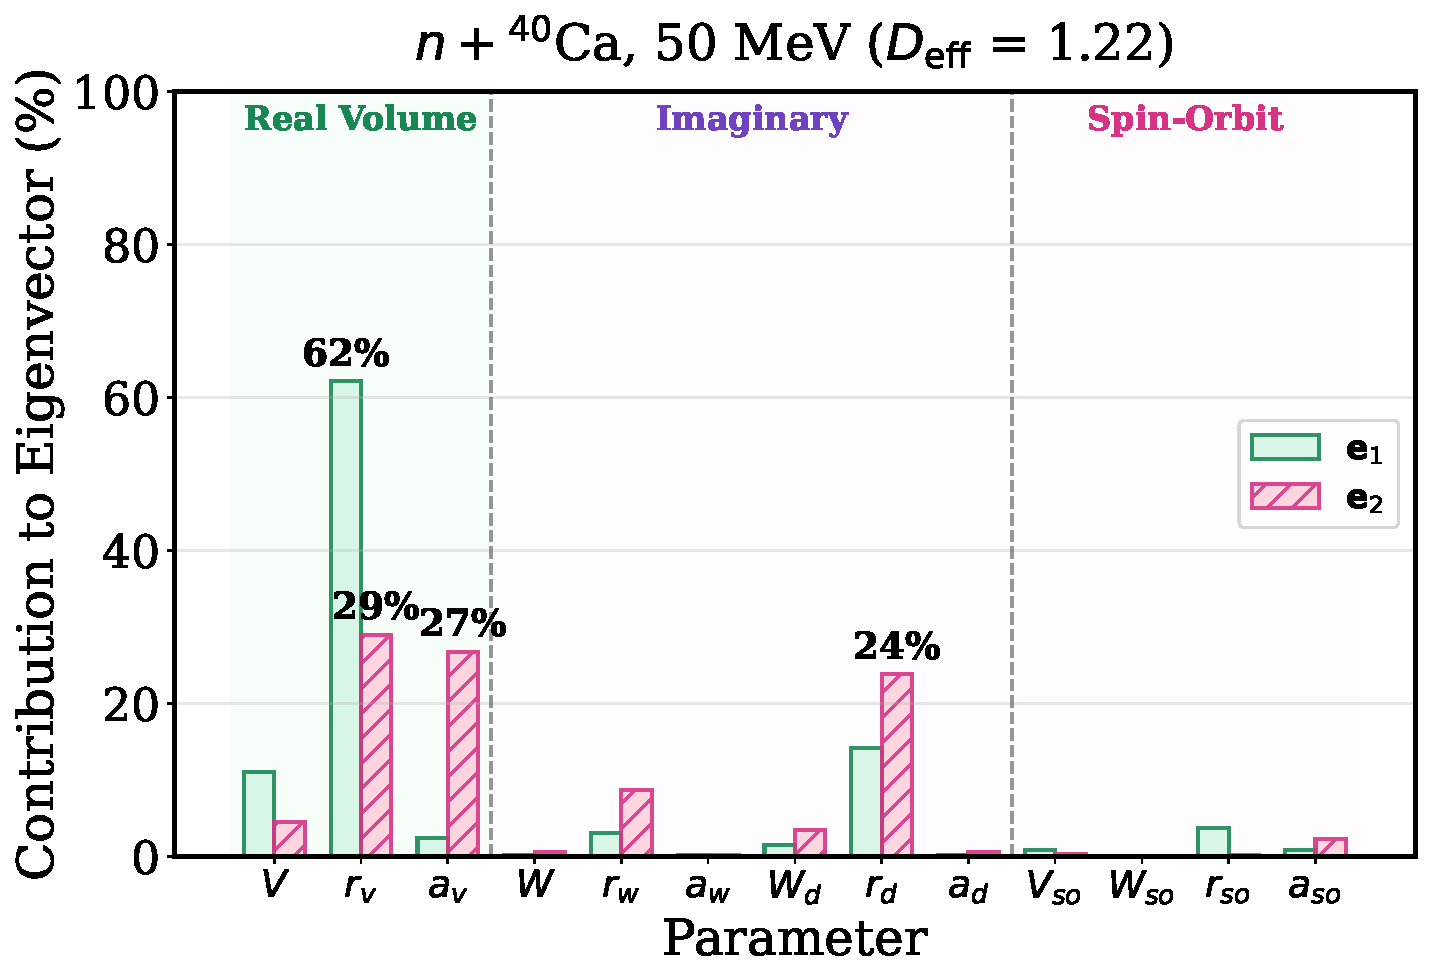
\includegraphics[width=\columnwidth]{fig3_eigenvectors.pdf}
\caption{Eigenvector composition for elastic $n+^{40}$Ca at 50~MeV (13 parameters). The ``potential radius'' mode $\mathbf{e}_1$ (green) is dominated by $r_v$ (62\%) with $r_d$ (14\%) and $V$ (11\%); the ``radial geometry'' mode $\mathbf{e}_2$ (rose) mixes $r_v$ (29\%), $a_v$ (27\%), and $r_d$ (24\%). Together they capture 97\% of the information.}
\label{fig:eigenvectors}
\end{figure}

The normalized sensitivity directions $\hat{S}_V(\theta)$ and $\hat{S}_{r_v}(\theta)$ overlap almost perfectly at all angles (see End Matter, Fig.~\ref{fig:sensitivity}), directly manifesting the Igo proportionality: fractional changes in $V$ and $r_v$ produce nearly indistinguishable effects on $d\sigma/d\Omega$. But can additional observables lift this degeneracy?

%=====================================================
% STEP-BY-STEP
%=====================================================
\textit{Step-by-step constraint analysis.}---I track how independent parameter directions open as information sources are progressively added (Fig.~\ref{fig:stepwise}).

\emph{Step 1: Elastic $d\sigma/d\Omega$ alone.}---For $n+^{40}$Ca at 50~MeV with 35 angular data points, $D_\mathrm{eff} = 1.22$ (an illustrative case; the 168-configuration average is $1.7 \pm 0.4$). Only the ``potential radius'' mode is constrained; the eigenvalue spectrum drops by nearly eight orders of magnitude.

\emph{Step 2: Adding $\sigma_R$.}---One additional datum, overwhelmed by 35 angular data points: $D_\mathrm{eff}$ increases by less than 0.001.

\emph{Step 3: Adding $A_y$.}---The analyzing power probes spin-orbit interference through the spin-flip amplitude $g(\theta)$. Adding $A_y$ raises $D_\mathrm{eff}$ from 1.22 to 1.53 for $n+^{40}$Ca, and from 1.15 to 1.72 for $n+^{120}$Sn (with the observable weighting defined in Method; the gain at experimental precision ratios is smaller, see End Matter). Within the present absolutely-normalized setup, integrated cross sections ($\sigma_R$, $\sigma_T$) provide no measurable additional gain.

\emph{Step 4: Systematic multi-energy fitting.}---The combined Fisher matrix is constructed by projecting each single-energy $F(E)$ onto the shared KD02 global coefficients via the Jacobian $J(E) = \partial\boldsymbol{\theta}_\mathrm{local}(E)/\partial\boldsymbol{\theta}_\mathrm{global}$ and summing $F_\mathrm{global} = \sum_E J^T F(E) J$, then projecting back to the local space at a reference energy, $F_\mathrm{ref} = J(E_\mathrm{ref})\,F_\mathrm{global}\,J(E_\mathrm{ref})^T$ (the back-projection is convention-dependent; see End Matter). Combining 7 energies (10--200~MeV) with elastic data alone raises $D_\mathrm{eff}$ to 2.47 ($n+^{40}$Ca) and 2.19 ($n+^{120}$Sn), the largest single improvement, exploiting the energy lever arm: real potential dominates at low energy, absorption at high energy. Including all observables gives $D_\mathrm{eff} = 2.16$ (Ca) and 2.27 (Sn); the combined value can fall below or above the elastic-only one, depending on whether $A_y$ concentrates or broadens the spectrum for that system (see End Matter). This gain relies jointly on the additional data \emph{and} the KD02 energy dependence that ties parameters across energies.

\emph{Step 5: KD02 global systematics.}---The KD02 global model parametrizes each local potential parameter as a function of mass $A$, charge $Z$, and energy $E$ through 48 universal coefficients (9 shared geometry, 16 shared depth, 10 neutron-specific, and 13 proton-specific; see End Matter, Table~\ref{tab:kd02_params}). Projecting the 168 single-system Fisher matrices onto this universal space via the Jacobian $J_i = \partial\log\boldsymbol{\theta}_\mathrm{local}/\partial\log\boldsymbol{\theta}_\mathrm{universal}$ and summing (see End Matter, Fig.~\ref{fig:global_fisher}) yields $D_\mathrm{eff} = 2.9$ (out of 48), with the dominant eigenvector (44\% of information) mixing $r_{v0}$ (70\%) and $r_{so,0}$ (24\%). With neutron data alone, $D_\mathrm{eff}$ peaks at $\sim$3.1 after the first few systems and settles near 3.0; adding proton data leaves the final value essentially unchanged (2.9), because protons largely reinforce the same dominant directions rather than opening new ones. The Igo ambiguity governs the global constraint structure.

\begin{figure}[t]
\centering
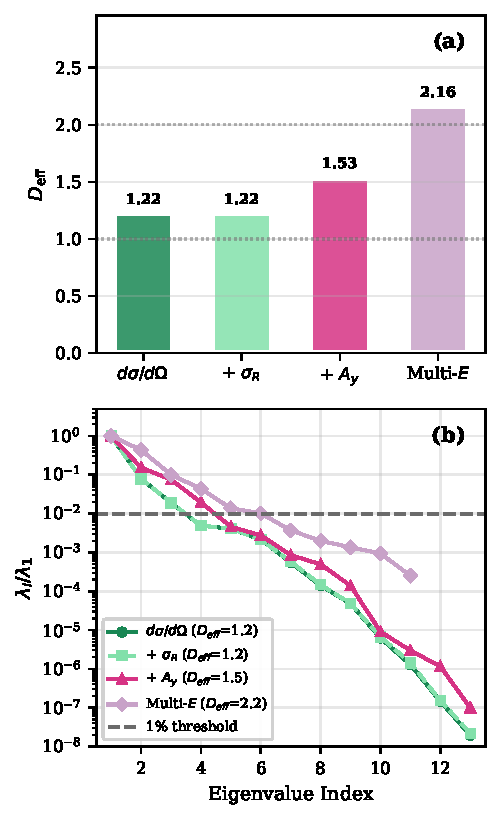
\includegraphics[width=\columnwidth]{fig_stepwise.pdf}
\caption{Step-by-step constraint analysis for $n+^{40}$Ca. (a)~$D_\mathrm{eff}$ for 13 local parameters increases as observables and energies are added (Steps 1--3 at 50~MeV; Step~4 combining 7 energies 10--200~MeV via Jacobian projection through the KD02 universal coefficient space): elastic alone (1.22), $+\sigma_R$ (no change), $+A_y$ (1.53), multi-energy with all observables (2.16). (b)~Eigenvalue spectra at each step. The multi-energy curve has 11 non-zero eigenvalues because the KD02 constraints $r_w = r_v$ and $a_w = a_v$ eliminate 2 of the 13 local degrees of freedom.}
\label{fig:stepwise}
\end{figure}


%=====================================================
% CONNECTION TO BAYESIAN ANALYSIS
%=====================================================
\textit{Connection to Bayesian analysis.}---The Fisher information matrix makes the empirical findings of King \textit{et al.}~\cite{King2019PRL} quantitative. In the Gaussian (Laplace) approximation~\cite{Sivia2006}, the posterior covariance equals $\Sigma_\mathrm{post} = F^{-1}$, so the eigenvector decomposition (Fig.~\ref{fig:eigenvectors}) predicts what their MCMC sampling found: $\mathbf{e}_1$, dominated by $r_v$ and $V$ with the same sign (the volume integral direction), produces precisely the elongated $V$-$r_v$ correlation they observed, while the remaining parameters contribute to sloppy directions whose correlations stay invisible in finite MCMC samples; the extreme eigenvalue hierarchy likewise explains the spurious frequentist correlations noted in the Introduction (see End Matter for the eigenvalue ranges and the projection mechanism). The two approaches are complementary: Fisher maps the global constraint structure with $\sim$3700$\times$ fewer evaluations, while MCMC captures non-Gaussian features.

%=====================================================
% DISCUSSION AND CONCLUSION
%=====================================================
\textit{Discussion and Conclusion.}---The results above answer the three questions posed in the Introduction. (1)~Within the KD02 optical model framework, single-energy elastic scattering constrains only $D_\mathrm{eff} \approx 1.7$ out of 13 parameter combinations; systematic multi-energy fitting raises $D_\mathrm{eff}$ to only $\sim$2.3--2.5 on average (up to $\sim$3 for the lightest systems) in the 13-parameter local space, and $D_\mathrm{eff} \approx 2.9$ out of 48 in the universal coefficient space. (2)~Within the local Fisher description, uniform error reduction rescales all eigenvalues without changing their participation ratio: $D_\mathrm{eff}$ measures the shape of the spectrum, not its total magnitude. Breaking the bottleneck therefore requires data that probe qualitatively different directions (systematic multi-energy fitting, spin observables), not simply smaller errors within the same error model. This is consistent with long-standing practice: physical interpretations of optical-model parameters are supplied by additional observables and by model structure, through matter densities folded with an effective nucleon-nucleon interaction~\cite{Greenlees1968} or dispersive relations linking real and imaginary parts across energies~\cite{Mahaux1991}. These inputs can constrain combinations that an isolated angular distribution leaves flat. A direct nucleon-nucleus example is the nonlocal dispersive analysis of $^{40}$Ca: local and nonlocal absorptive potentials reproduce equivalent elastic differential cross sections but give different angular-momentum absorption profiles, and only the nonlocal form also recovers particle number and charge density~\cite{Mahzoon2014}. The resulting constraints on Woods-Saxon radii, diffusenesses, and depths remain conditional on the assumed density, folding interaction, dispersive ansatz, or global energy dependence, rather than being model-independent information contained in one angular distribution. The observable-class dependence found here has a well-known heavy-ion counterpart, where fusion and elastic scattering demand incompatible Woods-Saxon diffuseness values~\cite{Newton2004}. (3)~Within the KD02 framework, the information bottleneck is stable: $D_\mathrm{eff}$ shows only weak dependence on target mass ($A = 12$--$208$), beam energy (10--200~MeV), and projectile type, and persists in the full 48-dimensional universal coefficient space ($D_\mathrm{eff} = 2.9$ out of 48). This behavior traces to the surface-dominated scattering produced by the short-range nuclear force: the near-collinearity of the normalized sensitivity directions $\hat{S}_V$ and $\hat{S}_{r_v}$ at all angles (Fig.~\ref{fig:sensitivity}) is a consequence of the $J_V \propto V r_v^3$ structure shared by Woods-Saxon-type local potentials; verification with other global parameterizations is a natural extension.

The step-by-step decomposition sets a measurement priority for opening independent parameter directions: multi-energy fitting gives the largest increase from the elastic baseline ($\Delta D_\mathrm{eff} = 1.24$ and 1.03 for $n+^{40}$Ca and $n+^{120}$Sn, compared to 0.31 and 0.56 from $A_y$ at the Method weighting, all computed from the unrounded single-energy $D_\mathrm{eff}$ values), while in the median $A_y$ opens more independent structure than $\sigma_R$ at a single energy (the quantitative change depends on $\epsilon/\delta_{A_y}$; see End Matter). This is a ranking of spectral broadening, not of total Fisher information, which can increase even when $D_\mathrm{eff}$ decreases. For rare-isotope beam facilities~\cite{Hebborn2023,Hebborn2023PRL} where beam time is precious, the results favor distributing measurements across energies when the goal is to separate parameter directions rather than only to tighten an already-stiff combination.

In logarithmic KD02 coordinates, these results exhibit the standard local Fisher-spectrum signature of a ``sloppy model.'' The same Fisher analysis also applies to nucleon-nucleon potentials and chiral effective field theory, where the low-energy constants play the role of the optical potential parameters. Microscopic optical potentials from ab initio theory offer a path to bypass the parametric degeneracy entirely, by constraining the potential from nuclear forces rather than from scattering data alone. In practical terms, an elastic fit with a small $\chi^2$ does not by itself determine the optical input needed for a transfer or breakup calculation; the unconstrained directions must either be pinned by external physics or propagated as uncertainty to the reaction observable. The $D_\mathrm{eff}$ values established here provide a benchmark within the stated coordinates and error models: any potential whose observables share a similar sensitivity geometry will face a comparable information bottleneck when constrained by scattering data alone.

%=====================================================
\begin{acknowledgments}
This work was supported by the National Natural Science Foundation of China (Grant Nos.~12475132 and 12535009) and the Fundamental Research Funds for the Central Universities.

In accordance with the APS policy on the appropriate use of AI tools, I disclose the following substantive AI assistance: large-language-model assistants, Claude (Anthropic, Opus~4 series, via Claude Code) and Codex (OpenAI, GPT-5 series), were used to assist with developing and debugging the analysis code, to provide separate numerical cross-checks (including a verification pass in which every quoted number was recomputed from the analysis scripts and the partial-wave convergence of the Fisher derivatives was certified), and to revise the manuscript text. All physics formulations, analysis choices, and conclusions are my own. I directed each use, checked numerical outputs against the archived analysis scripts and data, reviewed all text revisions against the manuscript record and cited sources, and take full responsibility for the entire content.
\end{acknowledgments}

\bibliography{references}

% =====================================================
% PRL End Matter, placed after references in publication
% =====================================================
\onecolumngrid
\bigskip
\begin{center}
\rule{0.5\columnwidth}{0.5pt}\\[6pt]
{\large\textbf{End Matter}}\\[6pt]
\rule{0.5\columnwidth}{0.5pt}
\end{center}
\twocolumngrid

\textit{Numerical method.}---The Schr\"odinger equation for each partial wave is solved using the Numerov algorithm with matching to Coulomb functions at large radius. The partial-wave sum uses $l_\mathrm{max} = kR + 50$ with $R = 1.25\,A^{1/3}$~fm; repeating the full 168-configuration scan with fixed $l_\mathrm{max} = 90$ and 120 changes $D_\mathrm{eff}$ by at most 0.012. For spin-1/2 scattering, the solver iterates over all $(l, j)$ partial wave channels, with the spin-orbit potential entering through the Thomas form with factor of 2 ($\mathbf{l}\cdot\boldsymbol{\sigma} = 2\mathbf{l}\cdot\mathbf{s}$). From the $(l,j)$-resolved $S$-matrix, the direct and spin-flip scattering amplitudes $f(\theta)$ and $g(\theta)$ are constructed, yielding $d\sigma/d\Omega = |f|^2 + |g|^2$, $A_y = 2\mathrm{Im}(fg^*) / (|f|^2 + |g|^2)$, $\sigma_R$, and $\sigma_T$. Parameter sensitivities are computed using two-point central finite differences with step size $\delta = 0.01\,|p_i|$, verified to be fully converged: scanning $\delta$ over three orders of magnitude ($10^{-5}|p_i|$ to $10^{-2}|p_i|$) changes $D_\mathrm{eff}$ by less than $0.2\%$, and a five-point stencil yields identical $D_\mathrm{eff}$ to three to four significant figures. All results use 35 equally spaced angles from $5^\circ$ to $175^\circ$; increasing to 50 or 90 angular points changes $D_\mathrm{eff}$ by less than 0.002. The solver has been validated against FRESCO~\cite{Thompson1988}, achieving $S$-matrix agreement to $|\Delta S| < 0.002$ and cross-section agreement to $< 0.2\%$.

\textit{Robustness checks.}---Four checks confirm that the conclusions are robust to analysis choices. (1)~\emph{Evaluation point}: Perturbing all 13 KD02 parameters simultaneously by $\pm 10\%$ around the reference values (10 random trials per system) yields $D_\mathrm{eff}$ in the range 1.1--2.5 for elastic scattering, with means within 0.25 of the reference values. The conclusion $D_\mathrm{eff} \ll N_p$ is robust to the choice of evaluation point. (2)~\emph{Geometry constraints}: Enforcing the KD02 constraints $r_w = r_v$ and $a_w = a_v$ (reducing from 13 to 11 free parameters) shifts the elastic $D_\mathrm{eff}$ by $-0.4$ to $+0.5$ across the 168 configurations (an increase in 115 of them; $+0.14$ to $+0.31$ for the representative 50~MeV systems), leaving the conclusion $D_\mathrm{eff} \ll N_p$ unchanged in either parameterization. (3)~\emph{Observable weighting}: The combined $D_\mathrm{eff}$ depends on $\epsilon / \delta_{A_y}$. A census over all 168 configurations shows that the $A_y$ gain is precision-dependent and neutron-dominated: at $\epsilon = 5\%$ ($\epsilon/\delta_{A_y} = 1.7$), adding $A_y$ raises $D_\mathrm{eff}$ in 113 of 168 configurations (neutrons 68/84, median gain $+0.16$; protons 45/84, median $\approx 0$), while at $\epsilon = 10\%$ the count drops to 92 of 168. Where $A_y$ lowers $D_\mathrm{eff}$, the added information makes the eigenvalue spectrum more peaked rather than opening balanced new directions (cf. the global analysis, Fig.~\ref{fig:global_fisher}). Adding $\sigma_R$ raises $D_\mathrm{eff}$ in all 168 configurations but with median gain $6\times10^{-4}$; the only gains above 0.05 occur for sub-barrier proton scattering ($p+^{197}$Au and $p+^{208}$Pb at 10~MeV), where the elastic angular distribution is Rutherford-dominated and constrains the absorptive parameters only weakly, so that $\sigma_R$ opens an absorption-sensitive direction. At representative precision ratios the median gains order as multi-energy $\gg$ $A_y$ $\gg$ $\sigma_R$. (4)~\emph{Back-projection convention}: The local-space multi-energy values of Step~4 use the stated map $F_\mathrm{ref} = J(E_\mathrm{ref})\,F_\mathrm{global}\,J(E_\mathrm{ref})^T$. Because $J$ is $13 \times 48$ with rank 11 (the KD02 constraints $r_w = r_v$, $a_w = a_v$), no unique inverse transformation exists and the back-projected $D_\mathrm{eff}$ is convention-dependent: propagating the pseudo-inverse covariance instead ($\Sigma_\mathrm{loc} = J\,F_\mathrm{global}^{+}\,J^{T}$, $F_\mathrm{eff} = \Sigma_\mathrm{loc}^{+}$) gives larger values on average (2.9 instead of 2.3 over the 24 projectile-nucleus combinations, larger in 23 of the 24, insensitive to the pseudo-inverse threshold over four orders of magnitude). Under both conventions the multi-energy combination remains the largest broadening of the constrained subspace (from a single-energy all-observable average of 1.6), and the 48-coefficient global result $D_\mathrm{eff} = 2.9$ involves no back-projection.

\begin{figure*}[t]
\centering
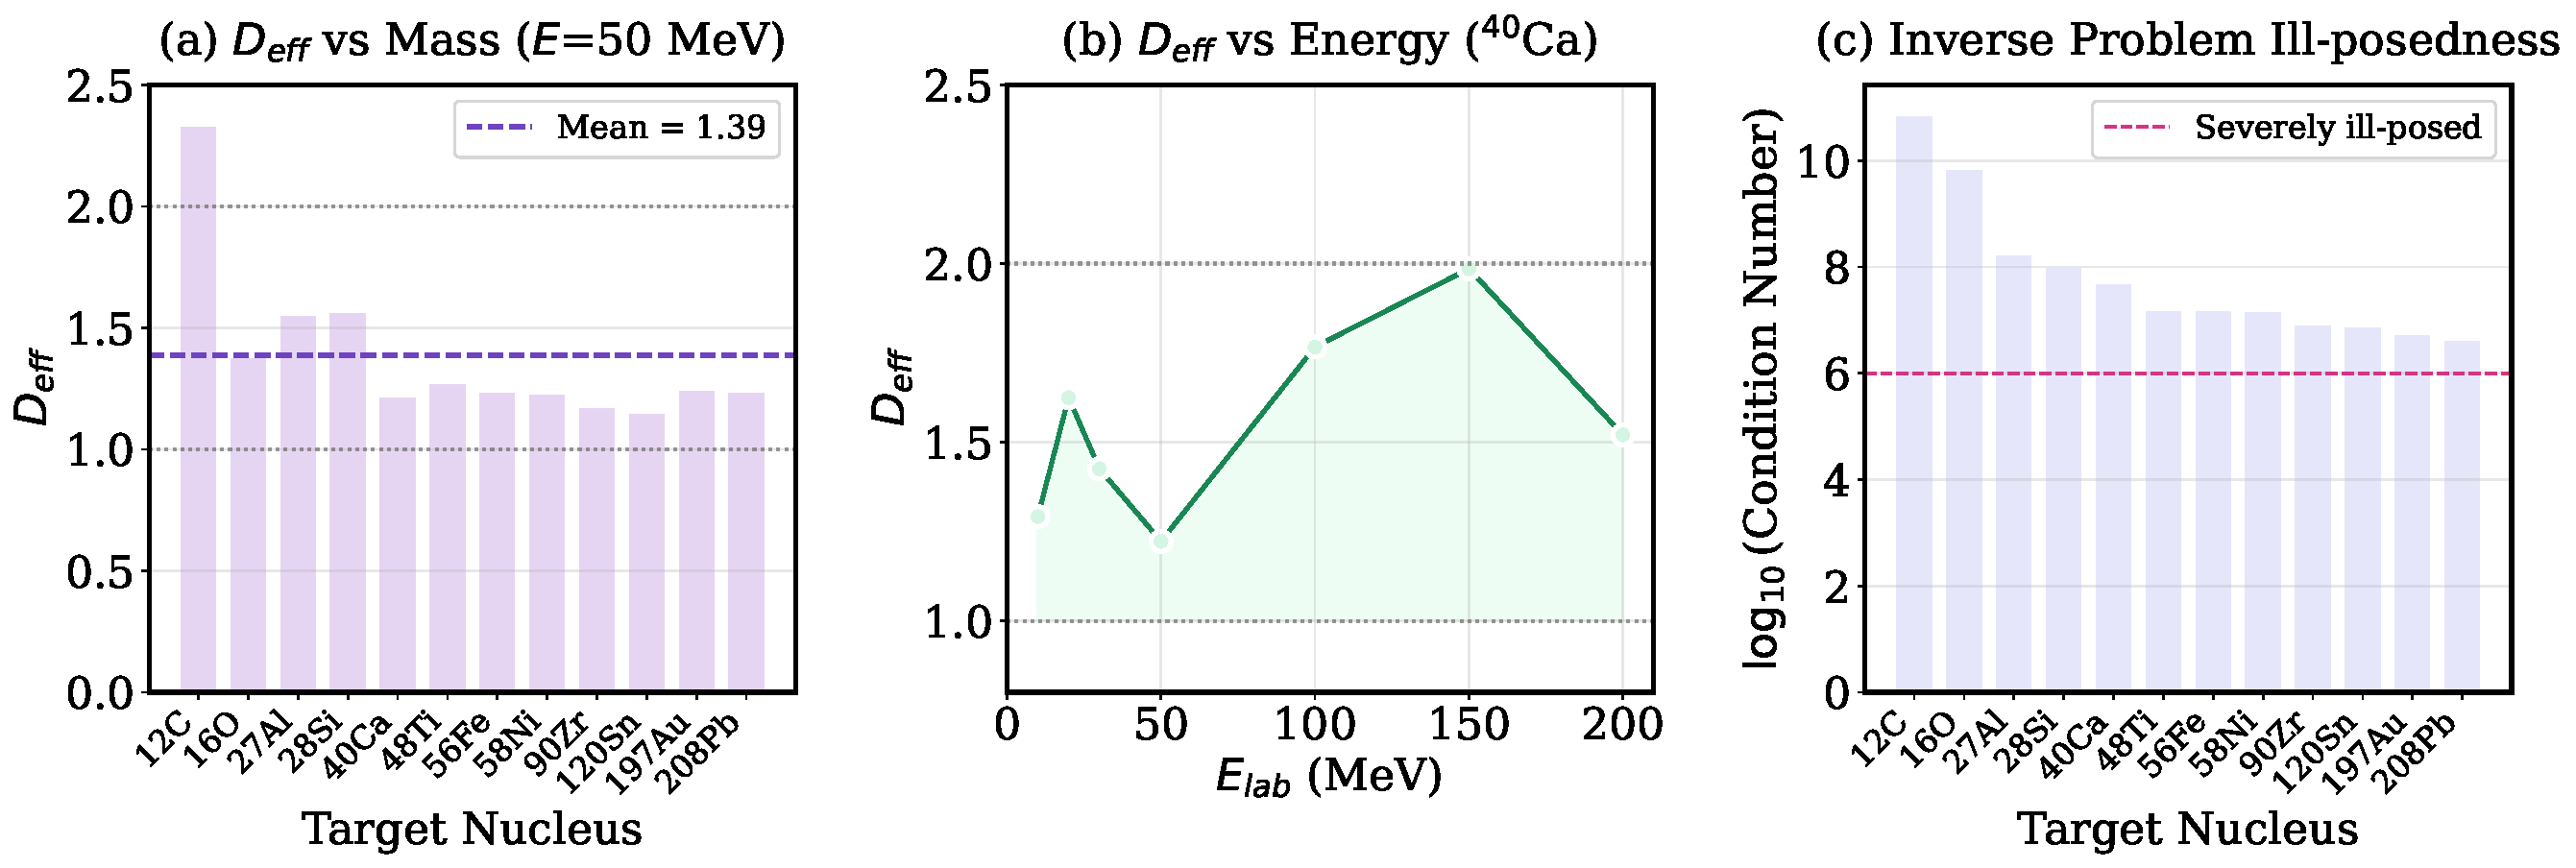
\includegraphics[width=\textwidth]{fig2_deff_combined.pdf}
\caption{Systematic analysis for $n+A$ scattering. (a)~$D_\mathrm{eff}$ versus mass at $E = 50$~MeV (neutrons only; mean lower than the all-energy, all-projectile average of $1.7 \pm 0.4$): $D_\mathrm{eff}$ stays within 1.1--2.4 across $A = 12$--$208$, largest for the lightest target. (b)~$D_\mathrm{eff}$ versus energy for $n+^{40}$Ca stays bounded. (c)~Condition number ranges from $10^6$ to above $10^{10}$, indicating extreme hierarchy between constrained and unconstrained directions.}
\label{fig:deff_combined}
\end{figure*}

\textit{Condition number and parameter extraction.}---The condition number $\kappa = \lambda_\mathrm{max}/\lambda_\mathrm{min}$ of the Fisher information matrix has a direct local interpretation for optical potential fitting. Consider $n+^{40}$Ca at 50~MeV, where $\kappa \approx 5 \times 10^7$. In the Gaussian approximation, the FIM eigenvalues are the inverse posterior variances along the principal axes, $\delta\theta_i \propto 1/\sqrt{\lambda_i}$, so the local precision ratio between the sloppiest and stiffest directions is $\sqrt{\kappa} \approx 7000$. This ratio is a diagnostic of the local anisotropy, not a claim that the quadratic approximation remains valid over a literal 7000\% displacement; establishing the global range requires a profile-likelihood or model-manifold calculation. Uniformly reducing the assumed errors rescales the local ellipsoid but leaves this axis ratio and $D_\mathrm{eff}$ unchanged.

This hierarchy also explains a familiar frustration in optical model fitting: $\chi^2$ minimizers converge rapidly along the stiff direction but wander erratically along sloppy directions, producing run-to-run variations in parameters like $a_v$ and $W$ even when the fitted cross sections are virtually identical. The FIM eigenvectors identify these ill-determined combinations explicitly, and could be used to reparameterize the fit in terms of stiff and sloppy coordinates, eliminating the numerical instability at its source.

\textit{KD02 parameter hierarchy.}---The KD02 potential involves parameters at two distinct levels.

\emph{Level 1: Local parameters (per system).}---At a specific $(A, Z, E)$ configuration, the potential is fully determined by 13 local parameters: real volume $(V, r_v, a_v)$, imaginary volume $(W, r_w, a_w)$, imaginary surface $(W_d, r_d, a_d)$, and spin-orbit $(V_{so}, W_{so}, r_{so}, a_{so})$. Of these, $r_w = r_v$ and $a_w = a_v$ in KD02, but I retain them as independent in the Fisher analysis to test whether data could distinguish them; the effect of enforcing these constraints (reducing to 11 parameters) is quantified in robustness check~(2) above. The single-energy Fisher matrix is $13 \times 13$.

\emph{Level 2: Universal coefficients (global model).}---The KD02 energy and mass dependence parametrizes each local parameter as a function of $A$, $Z$, and $E$ through analytical formulas with fitted numerical coefficients. For example, $E_f^n = -11.2814 + 0.02646\,A$ involves \emph{two} independent coefficients ($E_{f,0}^n$ and $E_{f,1}^n$), and $r_v = 1.3039 - 0.4054\,A^{-1/3}$ involves two more. Counting all such coefficients from Tables~10--11 and Eqs.~(25)--(26), (31)--(33), (36)--(37) of Ref.~\cite{Koning2003} yields 48 universal parameters. Table~\ref{tab:kd02_params} provides a complete accounting.

\begin{table}[h]
\caption{Complete inventory of KD02 universal coefficients, counted from Ref.~\cite{Koning2003}. Each coefficient is an independently fitted number in the global model. ``Shared'' parameters are identical for neutrons and protons.}
\label{tab:kd02_params}
\begin{ruledtabular}
\begin{tabular}{lcl}
Group & $N$ & Parameters \\
\hline
Shared geometry & 9 & $r_{v0}, r_{v1}$; $a_{v0}, a_{v1}$; $r_{d0}, r_{d1}$; \\
 & & $r_{so,0}, r_{so,1}$; $a_{so}$ \\
Shared depth & 16 & $v_{10}, v_{1,\mathrm{iso}}, v_{1A}, v_4$; $d_{10}, d_{1,\mathrm{iso}}$; \\
 & & $w_{20}, w_{21}$; $d_{20}, d_{2,\mathrm{amp}}, d_3$; \\
 & & $v_{so,10}, v_{so,11}, v_{so,2}$; $w_{so,1}, w_{so,2}$ \\
Neutron-specific & 10 & $E_{f,0}^n, E_{f,1}^n$; $v_{2,0}^n, v_{2,1}^n$; $v_{3,0}^n, v_{3,1}^n$; \\
 & & $w_{1,0}^n, w_{1,1}^n$; $a_{d,0}^n, a_{d,1}^n$ \\
Proton-specific & 13 & $E_{f,0}^p, E_{f,1}^p$; $v_{2,0}^p, v_{2,1}^p$; $v_{3,0}^p, v_{3,1}^p$; \\
 & & $w_{1,0}^p, w_{1,1}^p$; $a_{d,0}^p, a_{d,1}^p$; $r_{c,0}, r_{c,1}, r_{c,2}$ \\
\hline
Total & 48 & \\
\end{tabular}
\end{ruledtabular}
\end{table}

The distinction between levels matters physically. The full dataset of 168 configurations (12 nuclei $\times$ 7 energies $\times$ 2 projectiles) probes the 48 universal coefficients, yielding $D_\mathrm{eff} \approx 2.9$ (out of 48). Combining different nuclei adds constraining power through the $A$-dependence of geometry parameters, but the Igo ambiguity still dominates: the dominant eigenvector of $F_\mathrm{universal}$ is 70\% $r_{v0}$ and 24\% $r_{so,0}$, both radius coefficients.

\textit{Relation to Bayesian analysis.}---Here I provide additional technical details for the Fisher-Bayesian comparison discussed in the main text. King \textit{et al.}~\cite{King2019PRL}, analyzing nucleon-$^{48}$Ca, $^{90}$Zr, and $^{208}$Pb elastic scattering with 9 free central parameters (fixing spin-orbit), found that:
\begin{itemize}
\item Only the depth $V$ and radius $r$ of the real potential showed strong correlation in MCMC scatter plots;
\item All other parameter pairs exhibited approximately circular (uncorrelated) scatter plots;
\item The frequentist $\chi^2$ approach produced spurious strong correlations among many parameter pairs;
\item The frequentist 95\% confidence intervals were unrealistically narrow (44--92\% empirical coverage versus the nominal 95\%).
\end{itemize}

The eigenvalue hierarchy accounts for these observations quantitatively: the sloppy directions carry eigenvalues roughly 50 to $5\times10^7$ times smaller than $\lambda_1$, too small for finite MCMC sampling to resolve the associated correlations. The condition number of $10^6$ or larger [Fig.~\ref{fig:deff_combined}(c)] also explains the spurious frequentist correlations: projecting an anisotropic ``cigar-shaped'' posterior onto a Gaussian tangent plane creates artificial coupling between the elongated and compressed directions.

The narrow frequentist confidence intervals (Table~I of Ref.~\cite{King2019PRL}) are predicted by the Fisher analysis. The frequentist approach samples from the Gaussian approximation $\boldsymbol{\theta} \sim \mathcal{N}(\hat{\boldsymbol{\theta}}, F^{-1})$, valid only near the minimum. But with $D_\mathrm{eff} \approx 1.7$, the $\chi^2$ surface has $\sim$11 nearly flat directions where the Gaussian approximation breaks down, causing the frequentist method to underestimate the true parameter uncertainty along sloppy directions.

\textit{Computational advantages.}---The Fisher approach offers several practical advantages over Bayesian MCMC for systematic studies:
\begin{enumerate}
\item \emph{Efficiency}: Computing $D_\mathrm{eff}$ for one system requires $2N_p + 1 = 27$ evaluations of the scattering solver (for $N_p = 13$), taking a few seconds per configuration. King \textit{et al.} required $\sim$100,000 MCMC samples per system for converged parameter correlations. The $\sim$3700-fold speedup enables the systematic scan across 168 configurations, an analysis that would require $\sim$$10^7$ total solver calls with MCMC.
\item \emph{Analytical results}: The scale-invariance of $D_\mathrm{eff}$ (invariance under $F \to \alpha F$) is an exact mathematical property, whereas establishing this from MCMC would require running chains at multiple noise levels.
\item \emph{Decomposability}: The Fisher matrix can be additively decomposed by observable ($F = F_\mathrm{elastic} + F_{A_y} + F_{\sigma_R} + \cdots$) at each energy, and combined across energies via the Jacobian projection $F_\mathrm{global} = \sum_E J(E)^T F(E)\, J(E)$ that accounts for the KD02 energy dependence (Step~4), enabling the step-by-step analysis in Fig.~\ref{fig:stepwise}. Bayesian posteriors cannot be similarly decomposed without re-running the full MCMC.
\item \emph{Subgroup analysis}: Block sub-matrices of $F$ quantify the information content for parameter subgroups (real volume, imaginary, spin-orbit), providing physical insight into which observables constrain which parameters.
\end{enumerate}

A natural next step is to use the FIM eigenvectors to define an optimal reparameterization that separates stiff from sloppy directions, potentially improving MCMC convergence by orders of magnitude~\cite{Catacora2021}.

\textit{Multi-system global analysis.}---The per-nucleus KD02 analysis uses 13 local parameters specific to a given $(A, Z, E)$ configuration. A natural question is whether combining data from many nuclei and energies can break the information bottleneck. To address this, I extend the analysis to the full KD02 universal coefficient space: 48 parameters (Table~\ref{tab:kd02_params}) that generate all local potentials for any nucleus and energy through analytical prescriptions. These include shared geometry coefficients (e.g., $r_v = r_{v0} - r_{v1} A^{-1/3}$), energy-dependent depth amplitudes with Fermi-energy scales ($E_{f}^{n}$, $E_{f}^{p}$), and separate neutron/proton depth coefficients. For each of the 168 configurations (12 nuclei $\times$ 7 energies $\times$ 2 projectiles), the log-space Jacobian $J_i = \partial \log \boldsymbol{\theta}_\mathrm{local} / \partial \log \boldsymbol{\theta}_\mathrm{universal}$ transforms the local Fisher matrix into the universal space, and the combined Fisher matrix is obtained additively:
\begin{equation}
F_\mathrm{universal} = \sum_{i=1}^{168} J_i^T \, F_i^\mathrm{local} \, J_i.
\end{equation}

\begin{figure*}[htbp]
\centering
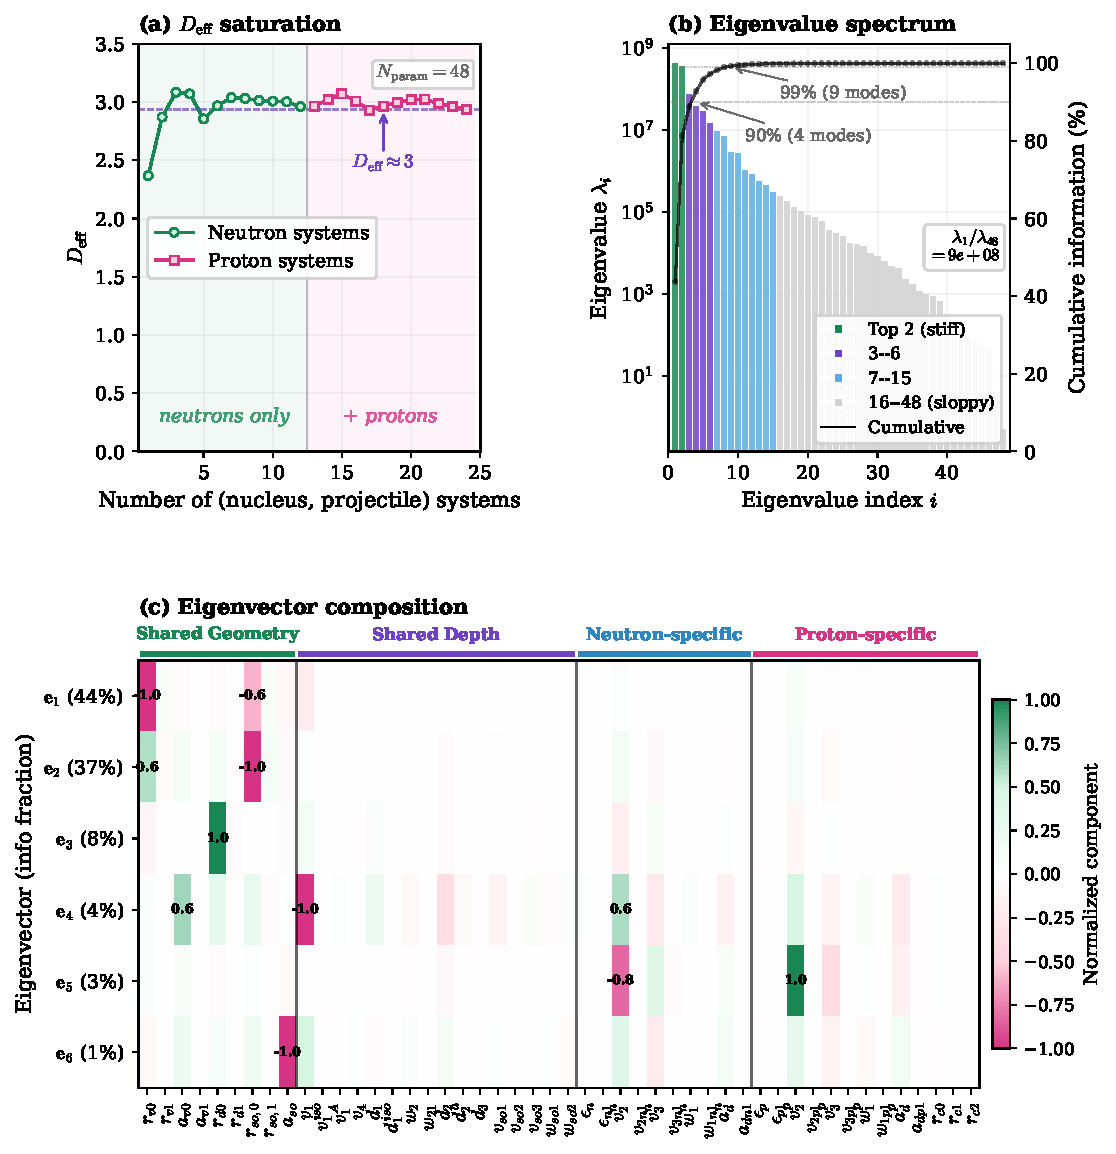
\includegraphics[width=\textwidth]{fig_global_fisher.pdf}
\caption{Global Fisher analysis in the 48-dimensional universal KD02 coefficient space. (a)~$D_\mathrm{eff}$ evolution as systems are added: neutron data (green) peak at $\sim$3.1 after the first few systems and settle near 3.0; adding proton data (pink) leaves the final value essentially unchanged ($\sim$2.9), because protons largely reinforce existing stiff directions rather than opening new ones. (b)~Eigenvalue spectrum: 4 modes carry over 90\% of all information, 9 modes suffice for 99\%, with condition number $\lambda_1/\lambda_{48} \approx 9 \times 10^8$. (c)~Eigenvector composition of the top 6 modes, with components normalized so that the largest absolute value in each row equals 1. The y-axis labels give the information fraction carried by each mode. See text for the squared-component decomposition ($|e_{i,k}|^2$) of each eigenvector.}
\label{fig:global_fisher}
\end{figure*}

The central result (Fig.~\ref{fig:global_fisher}) is that the information limit persists at the global level: $D_\mathrm{eff} = 2.9$ out of 48 universal parameters. Figure~\ref{fig:global_fisher}(a) shows the growth curve quoted in the main text: with neutron data alone $D_\mathrm{eff}$ rises sharply, peaks at $\approx$3.1 (three independent parameter directions constrained), and settles near 3.0; proton systems reinforce the same dominant directions (primarily $r_{v0}$) and make the eigenvalue spectrum more peaked, leaving the final value at 2.9. The entire nuclear chart of elastic scattering data thus constrains only $\sim$3 effective parameter combinations out of 48.

The eigenvalue spectrum [Fig.~\ref{fig:global_fisher}(b)] reveals an extreme hierarchy: the first eigenvalue $\lambda_1 = 4.2 \times 10^8$ carries 44\% of the total Fisher information, the second ($\lambda_2$, 37\%) and third ($\lambda_3$, 8\%) add progressively less, and the top 4 modes capture over 90\% of all information, while 9 modes reach 99\%. The remaining 39 eigenvalues share only $\sim$1\% of the total, spanning 9 orders of magnitude below $\lambda_1$. This near-singular structure means that the 48-dimensional parameter space is effectively collapsed to a $\sim$3-dimensional subspace by the data.

The eigenvector composition [Fig.~\ref{fig:global_fisher}(c)] reveals the physical identity of these constrained directions. The percentages below refer to squared components $|e_{i,k}|^2$, which give the fractional contribution of each parameter to a given mode (the figure displays the signed components, normalized so that the largest absolute value in each row equals 1). The dominant eigenvector $\mathbf{e}_1$ mixes $r_{v0}$ (70\%) and $r_{so,0}$ (24\%), the leading coefficients in the real-volume and spin-orbit radius parametrizations. The second eigenvector $\mathbf{e}_2$ reverses these weights ($r_{so,0}$ 69\%, $r_{v0}$ 25\%), while $\mathbf{e}_3$ is 91\% $r_{d0}$ (the surface imaginary radius). This confirms that the Igo ambiguity, which governs single-system fits, persists in the global constraint structure: elastic scattering across the nuclear chart primarily constrains the nuclear radius scale. All three leading modes are radius-dominated: scattering data constrain radii far more effectively than depths or diffusenesses.

Elastic-only data yield slightly \emph{higher} $D_\mathrm{eff}$ than the all-observable result. The reason is that $D_\mathrm{eff}$ measures the \emph{shape} of the eigenvalue spectrum (how uniformly information is distributed), not the total information content ($\mathrm{Tr}\,F$, which always increases with more data). Adding $A_y$ and $\sigma_R$ increases the leading eigenvalues by factors of roughly 250--500, but deposits this information along already-stiff directions (predominantly $r_{v0}$) rather than illuminating new sloppy directions. The eigenvalue distribution becomes more peaked and $D_\mathrm{eff}$ decreases. More data of the same kind therefore do not broaden the constrained subspace; data that probe different aspects of the potential do. Among the strategies tested in the main text (Fig.~\ref{fig:stepwise}), only systematic multi-energy fitting effectively opens new constraining directions, because different beam energies sample different radial regions of the potential.

\begin{figure}[htbp]
\centering
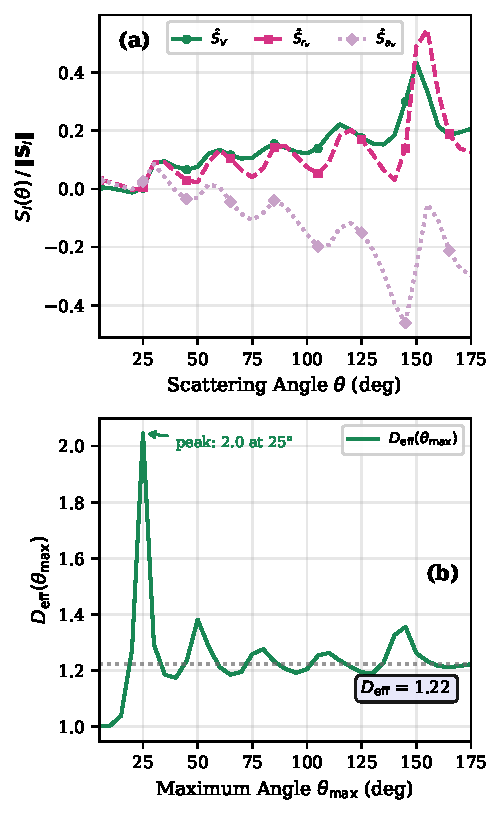
\includegraphics[width=\columnwidth]{fig_sensitivity_v2.pdf}
\caption{Angle-resolved sensitivity for $n+^{40}$Ca at 50~MeV. (a)~Normalized sensitivity directions $S_i(\theta)/\|\mathbf{S}_i\|$: overlapping curves indicate collinear (degenerate) parameter directions, while separated curves indicate independent information. $V$ (green) and $r_v$ (pink) overlap almost perfectly at all angles (Igo degeneracy). The diffuseness $a_v$ (lilac) also overlaps at forward angles but diverges at backward angles ($\theta \geq 100^\circ$), showing that $a_v$ develops an independent angular structure there. However, this independent component is small: 96\% of the squared norm of the backward-angle $a_v$ sensitivity lies in the $V$--$r_v$ plane (see text). (b)~Cumulative $D_\mathrm{eff}(\theta_\mathrm{max})$: peaks at $\sim$2.0 at $25^\circ$, on the approach to the first nuclear diffraction minimum (near $31^\circ$), where the steep angular variation briefly separates the sensitivity directions, then decreases as backward-angle data concentrates information along the dominant $V$--$r_v$ direction, settling to $D_\mathrm{eff} = 1.22$ at full coverage.}
\label{fig:sensitivity}
\end{figure}

\textit{Angle-resolved sensitivity and information geometry.}---To understand \emph{why} the information bottleneck arises, I examine the angular structure of parameter sensitivities. Figure~\ref{fig:sensitivity}(a) shows the normalized sensitivity directions $S_i(\theta)/\|\mathbf{S}_i\|$ for three parameters of the KD02 potential, computed for $n+^{40}$Ca at 50~MeV. Normalizing each sensitivity vector to unit length removes the overall magnitude and isolates the angular \emph{shape}: overlapping curves indicate collinear (degenerate) parameters, while separated curves indicate independent information content. Since $D_\mathrm{eff}$ is scale-invariant ($\epsilon^{-2}$ cancels in the participation ratio), this representation directly visualizes what determines $D_\mathrm{eff}$.

The normalized sensitivities $\hat{S}_V$ (green) and $\hat{S}_{r_v}$ (pink) overlap almost perfectly across all angles, a direct visualization of the Igo degeneracy~\cite{Igo1958}: fractional changes in $V$ and $r_v$ produce angular distributions that are nearly indistinguishable, making these two parameters impossible to separate from elastic scattering alone.

The diffuseness $\hat{S}_{a_v}$ (lilac) overlaps with $V$ and $r_v$ at forward angles ($\theta < 100^\circ$). At backward angles ($\theta \geq 100^\circ$), $a_v$ diverges and even changes sign, showing that diffuseness does develop an independent angular structure there. Because the Fisher matrix is built from logarithmic derivatives, the absolute magnitude of the cross section cancels in every matrix element, and backward-angle points are not down-weighted by their smaller cross sections; the root-mean-square logarithmic sensitivity of $r_v$ in fact grows from 5.7 at $\theta < 100^\circ$ to 16.5 at $\theta \geq 100^\circ$. The reason the independent structure of $a_v$ contributes little to $D_\mathrm{eff}$ is collinearity, not magnitude: 96\% of the squared norm of the backward-angle $a_v$ sensitivity lies in the plane spanned by $\mathbf{S}_V$ and $\mathbf{S}_{r_v}$, and the orthogonal remainder carries Fisher information of only $2\times10^{-3}$ of the leading eigenvalue $\lambda_1$. Restricting the Fisher matrix to backward angles alone gives $D_\mathrm{eff} = 1.20$, essentially identical to the forward-angle value of 1.19 and the full-coverage value of 1.22: the degeneracy is present in every angular region separately, rather than being an artifact of how the regions are weighted. The constraint on diffuseness comes primarily from multi-energy systematics (Step~4), not from backward-angle coverage at a single energy.

Figure~\ref{fig:sensitivity}(b) shows the cumulative effective dimensionality $D_\mathrm{eff}(\theta_\mathrm{max})$, computed from the Fisher matrix integrated over $\theta \in [5^\circ, \theta_\mathrm{max}]$. The curve is sharply non-monotonic: $D_\mathrm{eff}$ peaks at $\sim$2.0 at $\theta_\mathrm{max} = 25^\circ$, on the approach to the first nuclear diffraction minimum (located near $31^\circ$), where the steeply varying diffraction structure provides the most diverse constraints. As backward angles are included, information accumulates predominantly along the dominant $V$--$r_v$ direction, making the eigenvalue spectrum more peaked and reducing $D_\mathrm{eff}$. The final value $D_\mathrm{eff} = 1.22$ is reached at full angular coverage. This reveals an important subtlety: $D_\mathrm{eff}$ can temporarily \emph{exceed} its final value at restricted angular ranges, because the forward-angle diffraction pattern distributes information more uniformly across parameters than full-coverage data. Extending angular coverage increases the \emph{total} Fisher information ($\mathrm{Tr}\,F$) but concentrates it more heavily along the dominant direction, thereby reducing $D_\mathrm{eff}$.

\end{document}
